%
% Tutorial -- Modelling the 555 Timer.
%
% Copyright (C) 2006 Mike Brinson <mbrin72043@yahoo.co.uk>
%
% Permission is granted to copy, distribute and/or modify this document
% under the terms of the GNU Free Documentation License, Version 1.1
% or any later version published by the Free Software Foundation.
%

% redefine subfigure caption
\renewcommand{\thesubfigure}{\thefigure(\alph{subfigure})}
\makeatletter
  \renewcommand{\@thesubfigure}{\thesubfigure:\space}
  \renewcommand{\p@subfigure}{}
\makeatother

% redefine subtable caption
\renewcommand{\thesubtable}{\thetable(\alph{subtable})}
\makeatletter
  \renewcommand{\@thesubtable}{\thesubtable:\space}
  \renewcommand{\p@subtable}{}
\makeatother

\tutsection{Introduction}

The 555 timer was designed by Hans R. Camenzind in 1970\footnote{See "The 555 Timer IC. An interview with Hans Camenzind - The designer of the most successful integrated circuit ever developed", 
\url{http://semiconductormuseum.com/Transistors/LectureHall/Camenzind/} } and first produced by Signetics during the period 1971-1972\footnote{Now part of the Philips organisation.}. The device was originally called "The IC time machine" and given the part number SE555/NE555.   Over the last 30 plus years more than ten different semiconductor chip production companies have made 555 parts, making it one of the most popular ICs of all time\footnote{Recent manufacturing volumes indicate that the 555 timer is as popular as ever, with for example, Samsung (Korea) producing over one billion devices in 2003; see Wikipedia entry at  \url{http://en.wikipedia.org/}}.  Today it is still used in a wide range of circuit applications. 

\addvspace{12pt}

The 555 timer is one of the first examples of a mixed mode IC circuit that includes both analogue and digital components.
The primary purpose of the 555 timer is the generation of accurately timed single pulse or oscillatory pulse waveforms.  By adding one or two external resistors and one capacitor the device can function as a monostable or astable pulse oscillator. 

\addvspace{12pt}

The 555 timer is a difficult device to simulate. During circuit operation it switches rapidly between two very different DC states\footnote{Typically between ground and a voltage close to power rail VCC.}. Such rapid changes can be the cause of simulator DC convergence and transient analysis errors.  Most of the popular simulators include some form of 555 timer model, either built-in or as a subcircuit, which functions to some degree.  These models usually include a number of p-n junctions and non-linear controlled sources, making simulation times longer than those obtained with simpler models.  At the heart of the 555 timer are two comparators and a set-reset flip flop. A block diagram of the main functional elements that comprise the 555 timer is illustrated in Fig.~\ref{fig:555_timer_fig1}.  

\addvspace{12pt}

The current Qucs release does not include a model for the 555 timer.  The purpose of the work reported in this tutorial note has been to develop a 555 timer model from scratch which simulates efficiently, and is based only on the circuit components implemented in Qucs 0.0.10.  Moreover, while developing the Qucs 555 model every attempt has been made to reduce the number of p-n junctions to a minimum, yielding both model simplicity and reduced circuit simulation times.  The approach adopted is centred on established macromodelling techniques where signals at the timer device pins accurately model real device signals but internal macromodel signals often bare no relation to those found in an actual device.  Internally, the macromodel simply processes input signal information and outputs signals, in the correct format, to the device output pins.  In no way is an attempt made to simulate the actual 555 timer circuitry.

\begin{figure}[ht]
  \centering
  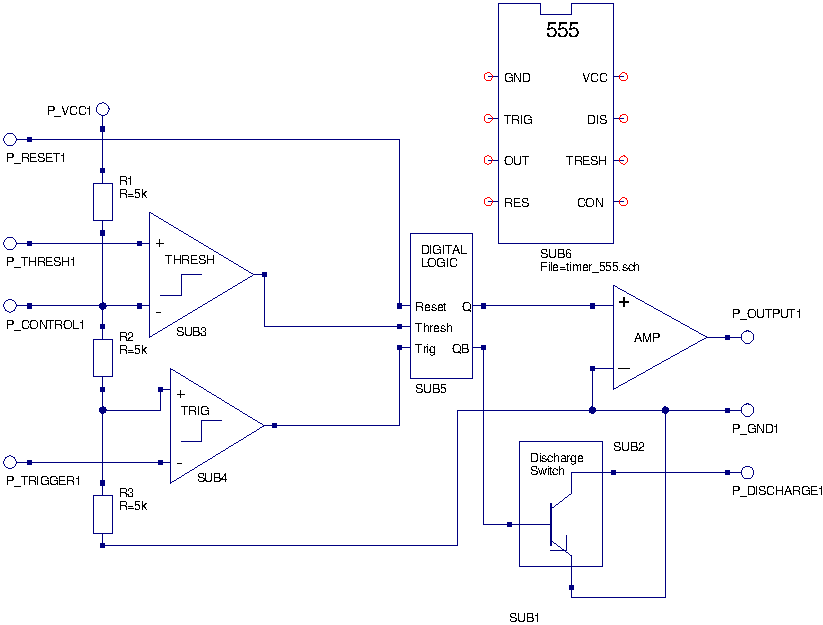
\includegraphics[width=0.9\linewidth]{555_timer_fig1}
  \caption{555 Timer functional block diagram.}
  \label{fig:555_timer_fig1}
\end{figure} 

\tutsection{The Qucs 555 timer model}

Fig.~\ref{fig:555_timer_fig1}  illustrates the new Qucs 555 timer model.  In this model each of the major functional blocks have been separated into macromodel subcircuits, grouping similar types of component together. Essentially, the model only includes standard Qucs components which all work together to produce the correct output signals through careful selection of threshold parameters, voltage limits, logic levels and rise and fall times.  These notes concentrate on explaining the structure and parameters of the macromodel subcircuits that form the 555 timer model, rather than describing the function of the device\footnote{A good tutorial guide to the operation of the 555 timer can be found at \url{http://www.uoguelph.ca/~antoon/gadgets/555/555.html}}. The 555 timer is an 8 pin device with:
\begin{itemize}
\item Pin 1 Ground    [GND]    - Most negative supply connected to the device, normally this is common ground (0V).
\item Pin 2 Trigger   [TRIG]   - Input pin to the lower comparator. Used to set the RS latch.
\item Pin 3 Output    [OUT]    - The 555 timer output signal pin.
\item Pin 4 Reset     [RES]    - Used to reset the RS latch.
\item Pin 5 Control   [CON]    - Direct access point to the (2/3)VCC divider node. Used to set the reference voltage for the upper comparator.
\item Pin 6 Threshold [THRESH] - Input pin to upper comparator. Used to reset the RS latch.
\item Pin 7 Discharge [DIS]    - Collector output of an npn BJT switch. Used to discharge the external timing capacitor.
\item Pin 8 VCC       [VCC]    - Most positive supply connected to device, normally this is 5V, 10V or 15V. 
\end{itemize}

\addvspace{12pt}

\tutsubsection{The trigger comparator macromodel}
The trigger comparator input pins are connected between the (1/3)VCC divider node and device package pin 2 (TRIG). Trigger input signals dropping below the (1/3)VCC divider node voltage cause the trigger output voltage to switch, setting the RS latch in the digital logic subcircuit.  This action also causes the 555 timer output signal to go high. The trigger input is level sensitive. Retriggering will occur if the trigger pulse is held low longer than the 555 timer output pulse width. The trigger comparator circuitry also has a storage time of several microseconds, limiting the minimum monostable output pulse to around 10$\mu$S. A DC current, popularly referred to as the trigger current, flows from device pin 2 (TRIG) into the external circuit. This has a typical value of 500 nA, setting the upper limit of resistance that can be connected from pin 2 to ground\footnote{At VCC = 5V this resistance is roughly 3.3M$\Omega$.}.  The circuit diagram of the trigger comparator macromodel is shown in Fig.~\ref{fig:555_timer_fig2}. The differential input signal is sensed by operational amplifier OP1. This has it's gain set to 1e6, giving a differential input signal resolution of 1$\mu$V. OP1 output voltages are limited to $\pm$1V. Note the upper +1V signal level corresponds to a logic '1' signal. Finally, the trigger comparator output voltage rise and fall times are set by time constant $R1*C1$. This network also adds a time delay to the comparator macromodel.
\FloatBarrier
\begin{figure}[ht]
  \centering
  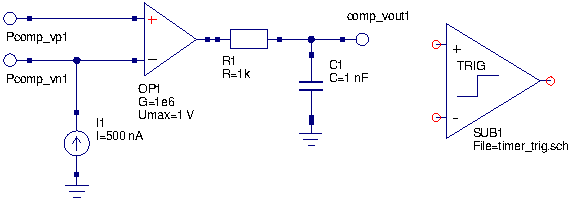
\includegraphics[width=0.9\linewidth]{555_timer_fig2}
  \caption{Trigger comparator macromodel.}
  \label{fig:555_timer_fig2} 
\end{figure} 
\FloatBarrier
\addvspace{12pt}

\tutsubsection{The threshold comparator macromodel} 
The threshold comparator macromodel is shown in Fig.~\ref{fig:555_timer_fig3}. It is very similar to the trigger comparator macromodel; one noteable difference is the size and direction of pin 6 (THRES) threshold DC current which is typically 100nA and flows into pin 6 from the external circuitry\footnote{The threshold DC current sets the upper limit to the value of the external resistor that can be connected between pin 6 and the VCC supply - for VCC = 5V this is approximately 16M$\Omega$, with VCC = 15 V this rises to roughly 20M$\Omega$.}. The threshold comparator is used to reset the RS latch in the 555 timer digital logic block, causing the 555 timer output to go low. Resetting occurs when the signal applied to external pin 6 (THRES) is driven from below to above the (2/3)VCC divider node voltage.  Again the threshold input is level sensitive.
\FloatBarrier
\begin{figure}[ht]
  \centering
  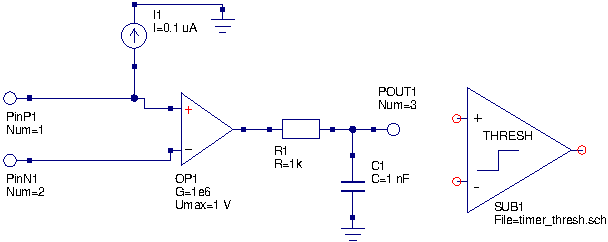
\includegraphics[width=0.9\linewidth]{555_timer_fig3}
  \caption{Threshold comparator macromodel.}
  \label{fig:555_timer_fig3} 
\end{figure} 
\FloatBarrier

\addvspace{12pt}



\tutsubsection{The digital logic macromodel}

The digital logic macromodel consists of an SR latch with additional combinational gates at the input of the model, see Fig.~\ref{fig:555_timer_fig4}.  The truth table for the SR latch is listed in Table~\ref{tab:tab1}.  All gates in the macromodel have logic '1' set at 1V and logic '0' set at 0V. RC timing networks have been added to the output of each gate, ensuring that the gates have a finite rise and fall times rather than the Qucs default value of zero seconds\footnote{In mixed mode circuit simulation transient analysis problems can occur when devices change state in zero seconds, see later notes for comments on this topic.}. Gate input signals with values less than the gate threshold voltage (0.5V) are considered to be a logic '0' signal. A logic '0' signal on 555 timer pin 4 (RES) also resets the SR latch causing the output signal, pin 3 (OUT), to move to a low state. The reset signal is an override signal in that it forces the timer output to a low state regardless of the signals on other timer input pins. Reset has a delay time of roughly 0.5$\mu$S, making the minimum reset pulse width of approximately 0.5$\mu$S. The reset signal is inverted then ORed with the threshold comparator output signal.  



\begin{table}
\centering
% use packages: array
\begin{center}
% use packages: array
\begin{tabular}{lllll}
Set (S) & Reset (R) & Q (P-Q1) & QB (P-QB1) & Notes \\ 
1 & 0 & 1 & 0 & Set state \\ 
0 & 0 & 1 & 0 &   \\ 
0 & 1 & 0 & 1 & Reset state \\ 
0 & 0 & 0 & 1 &  \\ 
1 & 1 & 0 & 0 & Undefined
\end{tabular}
\end{center}

\caption{Truth table for an SR latch constructed using NOR gates.}
\label{tab:tab1}
\end{table}
\FloatBarrier

\begin{figure}[ht]
  \centering
  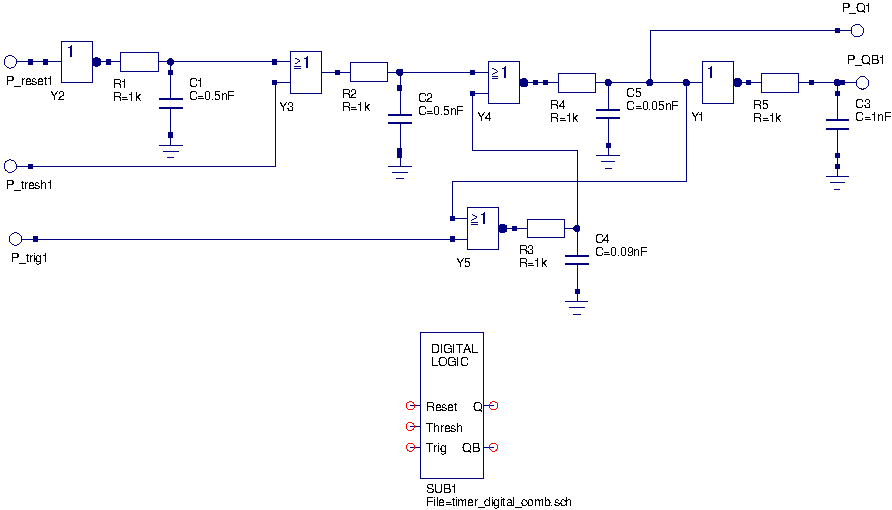
\includegraphics[width=1.05\linewidth]{555_timer_fig4}
  \caption{Digital logic macromodel.}
  \label{fig:555_timer_fig4} 
\end{figure} 
\FloatBarrier
\tutsubsection{The 555 timer output amplifier macromodel}

Illustrated in Fig.~\ref{fig:555_timer_fig5} is the macromodel for the timer output amplifier. This is a simple model constructed from a voltage gain block plus a resistor to represent the 555 timer output resistance.  The voltage gain block has it's value set to 3.5 in Fig.~\ref{fig:555_timer_fig5}.  This is the value needed to scale the logic '1' signal voltage to the required external voltage at timer output pin 3 (OUT). This value is only correct for power supply voltage VCC set to 5V, and must be changed for other voltages\footnote{At this time Qucs does not allow parameters to be passed to subcircuits, making it difficult to write generalised macromodels.  Adding parameter passing to subcircuits and the calculation of component values using equations is on the to-do list. Suggested values for the amplifier gain are: (1) VCC = 5V, G = 3.5, (2) VCC = 10V, G = 8.5V and (3) VCC = 15V, G = 13.5. These gain values correct for the voltage drop in the 555 timer totem-pole output stage.}. 
\FloatBarrier
\begin{figure}[ht]
  \centering
  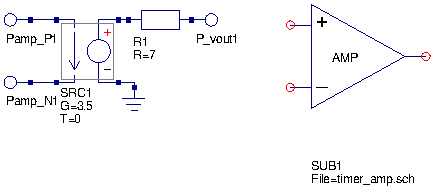
\includegraphics[width=0.8\linewidth]{555_timer_fig5}
  \caption{Output amplifier macromodel.}
  \label{fig:555_timer_fig5} 
\end{figure} 
\FloatBarrier

\tutsubsection{The discharge switch macromodel}
The discharge switch macromodel is shown in Fig.~\ref{fig:555_timer_fig6}. Like the actual 555 timer the macromodel discharge switch is based on an npn transistor.  A logic '1' signal applied to terminal \verb|pin_control_in1| turns the npn transistor on causing the path from the collector (555 timer pin DIS) to ground to become low resistance.  It is through this branch that the timer external capacitor is discharged. The reverse characteristic is observed when the input control voltage is logic '0'. In this case the collector to ground branch has a very high resistance. Resistor R1 is included in the macromodel to limit the npn base current when the BJT is turned on.  Similarly, resistor R2 has been added to the model to limit the external capacitor discharge current\footnote{Normally the external timing capacitor is discharged through a resistor in series with the collector to ground path.  However, if this series resistor is very small, or indeed does not exist, it is theoretically possible for the discharge current to become very large, which in turn leads to DC convergence errors or very long transient simulation times.}.
\FloatBarrier
\begin{figure}[ht]
  \centering
  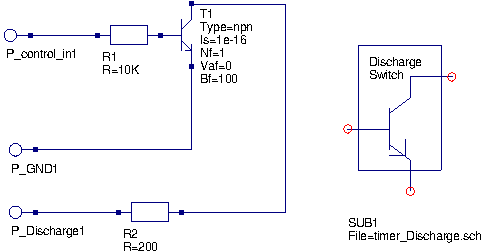
\includegraphics[width=0.8\linewidth]{555_timer_fig6}
  \caption{The discharge switch macromodel.}
  \label{fig:555_timer_fig6} 
\end{figure} 
\FloatBarrier


\tutsection{Published 555 timer test circuits}

The majority of manufacturers outline in their 555 timer specification sheets a range of fundamental circuit applications\footnote{See for example the "Applications Information" section of the National Semiconductor LM555 Timer data sheet, July 2006, www.national.com.}. A number of these circuits are introduced as a series of simulation test cases. The conditions chosen for the simulation tests are as follows:
\begin{itemize}
\item Integration method Gear, order 6 (this method works well with circuits that contain time constants that have widely different values)\footnote{One of the simulation tests also presents results using the standard trapezoidal second order integration method.}.
\item Input driver signals have a finite rise and fall time, usually in nano seconds (problems can occur when driver signals have either zero or very small rise and fall times - often a simulator will reduce the transient analysis step size in an attempt to reduce errors which in turn can significantly increase simulation run times).
\item Transient simulation parameter MinStep is set to one hundredth, or less, of the smallest rise or fall time in the circuit
(this is a good rule of thumb, giving reasonable simulation times and accuracy, normally without DC convergence or transient analysis time step problems).
\end{itemize}


\tutsubsection{The 555 timer monostable pulse generator}
Figure~\ref{fig:555_timer_fig7} shows the basic 555 timer monostable pulse generator circuit. The output pulse width is given by the equation $T=1.1*R5*C1 $; when $ R5 = 9.1k$ and $C1 = 0.01\mu F, T = 1ms$. Figure~\ref{fig:555_timer_fig8} illustrates the simulation waveforms for the monostable oscillator.

\FloatBarrier
\begin{figure}[ht]
  \centering
  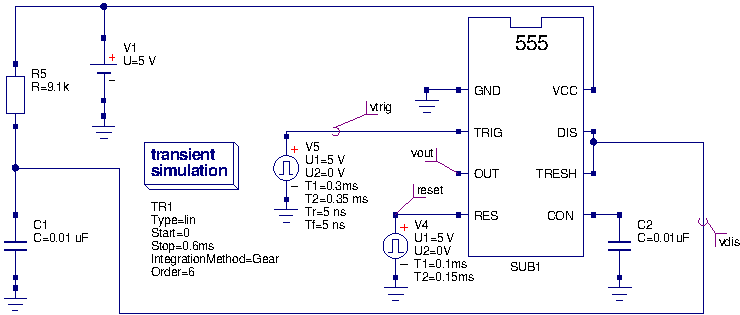
\includegraphics[width=1.0\linewidth]{555_timer_fig7}
  \caption{The basic 555 timer monostable pulse generator.}
  \label{fig:555_timer_fig7} 
\end{figure} 
\FloatBarrier
 
\FloatBarrier
\begin{figure}[ht]
  \centering
  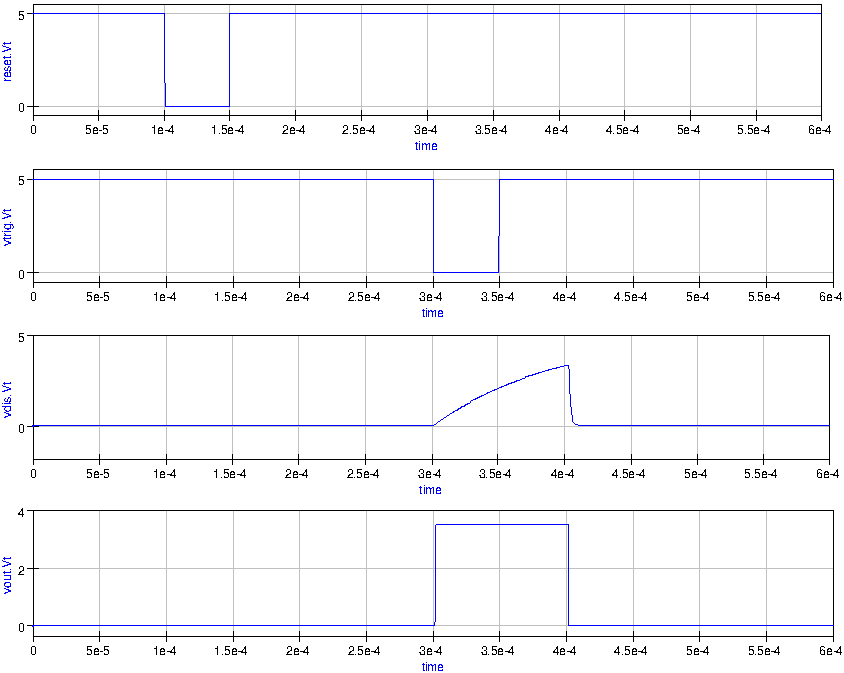
\includegraphics[width=1.0\linewidth]{555_timer_fig8}
  \caption{Simulation waveforms for the basic monostable pulse generator.}
  \label{fig:555_timer_fig8}  
\end{figure} 
\FloatBarrier

\tutsubsection{The 555 timer astable pulse oscillator}
Figure~\ref{fig:555_timer_fig9} shows the basic 555 timer astable pulse generator circuit. The charging time for capacitor C1 is given by $ tc = 0.693(R5+R6)C1$ seconds, and the discharge time by $ td = 0.693(R6)C1$ seconds. Hence, the period and frequency of oscillation are:\\
 $ T= tc + td = 0.693(R5 + 2R6)C1$ seconds, and $ f = \dfrac{1.44}{(R5+2R6)C1}$ Hz.\\

The duty cycle for the timer output waveform is also given by$ D = \dfrac{R6}{R5+2R6}$.\\

Figure~\ref{fig:555_timer_fig10} illustrates the simulation waveforms for the astable oscillator.
When resistor R6 is shunted by a diode, capacitor C1 charges via resistor R5 and discharges via resistor R6. On setting R5 = R6 a 50 percent duty cycle results\footnote{The value of R6 needs to be trimmed to set the duty cycle to exactly 50 percent.}, see Figures~\ref{fig:555_timer_fig11} and ~\ref{fig:555_timer_fig12}.

\FloatBarrier
\begin{figure}[ht]
  \centering
  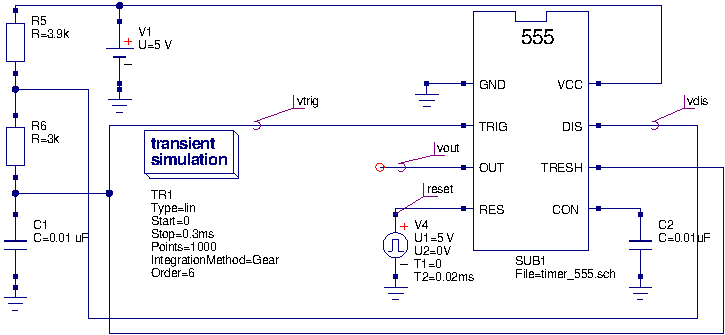
\includegraphics[width=1.0\linewidth]{555_timer_fig9} 
  \caption{The basic 555 timer astable pulse generator.}
  \label{fig:555_timer_fig9} 
\end{figure} 
\FloatBarrier

\FloatBarrier
\begin{figure}[ht]
  \centering
  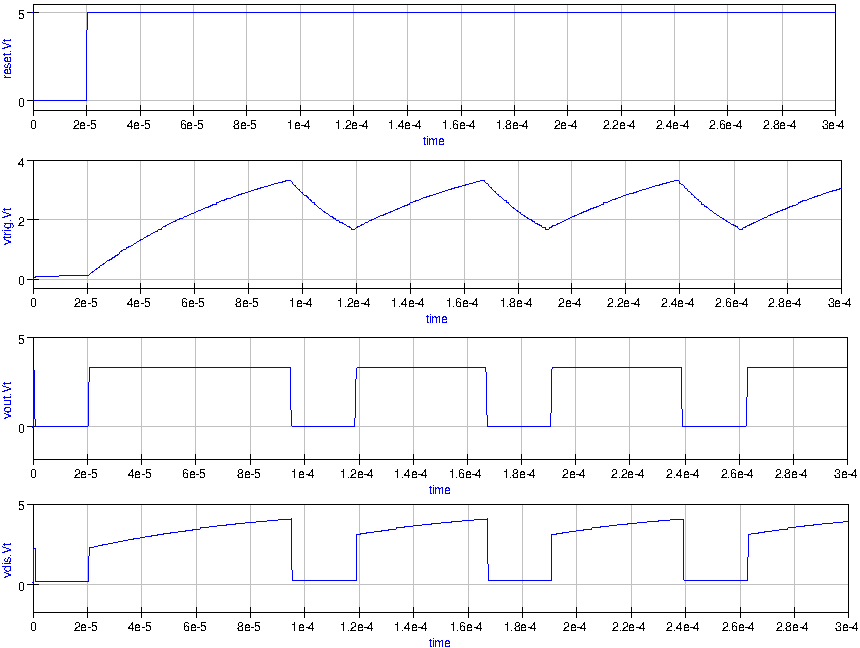
\includegraphics[width=1.0\linewidth]{555_timer_fig10}
  \caption{Simulation waveforms for the basic astable pulse generator.}
  \label{fig:555_timer_fig10} 
\end{figure} 
\FloatBarrier

\FloatBarrier
\begin{figure}[ht]
  \centering
  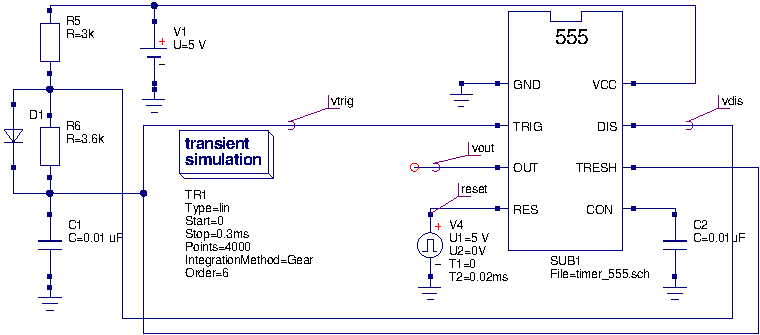
\includegraphics[width=1.0\linewidth]{555_timer_fig11}
  \caption{555 timer astable pulse generator with 50 percent duty cycle.}
  \label{fig:555_timer_fig11} 
\end{figure} 
\FloatBarrier

\FloatBarrier
\begin{figure}[ht]
  \centering
  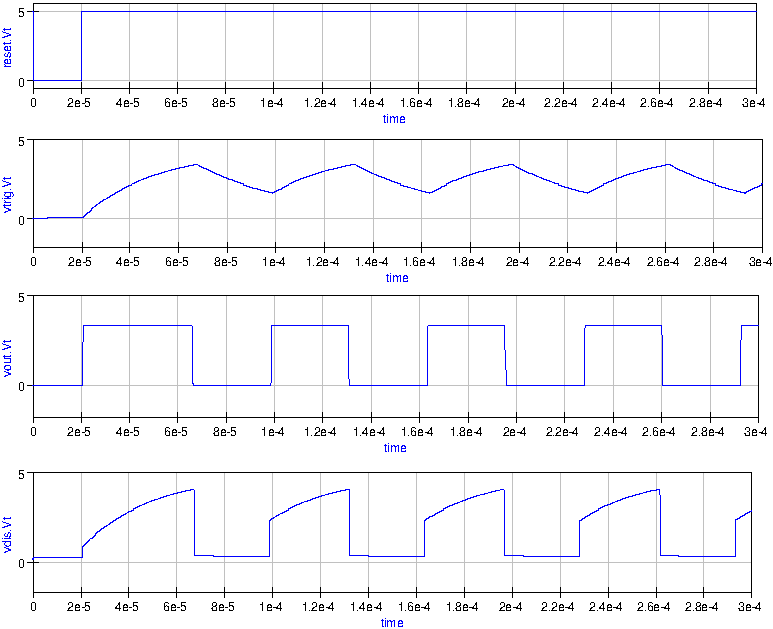
\includegraphics[width=1.0\linewidth]{555_timer_fig12}
  \caption{Simulation waveforms for 50 percent duty cycle astable pulse generator.}
  \label{fig:555_timer_fig12} 
\end{figure} 
\FloatBarrier

\tutsubsection{Pulse width modulation}

Triggering the 555 timer in monostable mode with a continuous sequence of pulses allows the output pulse width to be modulated by changing the amplitude of a signal applied to the control input pin 5 (CON). An example pulse width modulator circuit is given in Fig.~\ref{fig:555_timer_fig13}. In this circuit components C2, R6 and D1 convert the 555 trigger signal into a falling edge triggering signal.  This can be seen in Fig.~\ref{fig:555_timer_fig14} which illustrates the trigger, discharge and resulting output waveform. The 555 timer control pin is driven from a voltage pulse source. The specification of the control waveform has been chosen to generate a triangular shaped signal so that the modulation of the pulse width can be clearly seen as the control signal amplitude changes.

\FloatBarrier
\begin{figure}[ht]
  \centering
  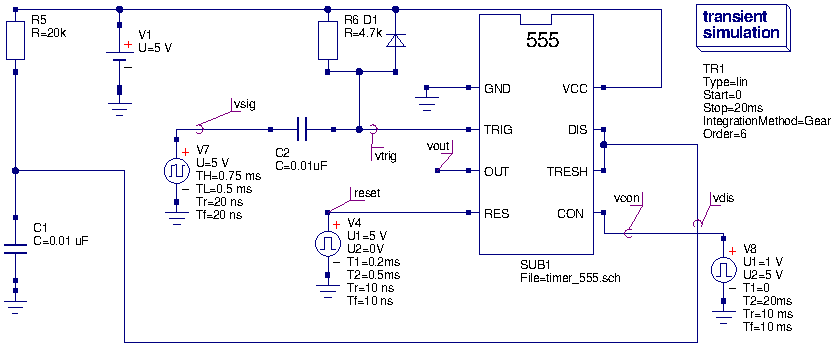
\includegraphics[width=1.0\linewidth]{555_timer_fig13}
  \caption{Pulse width modulator 555 timer circuit.}
  \label{fig:555_timer_fig13} 
\end{figure} 
\FloatBarrier

\FloatBarrier
\begin{figure}[ht]
  \centering
  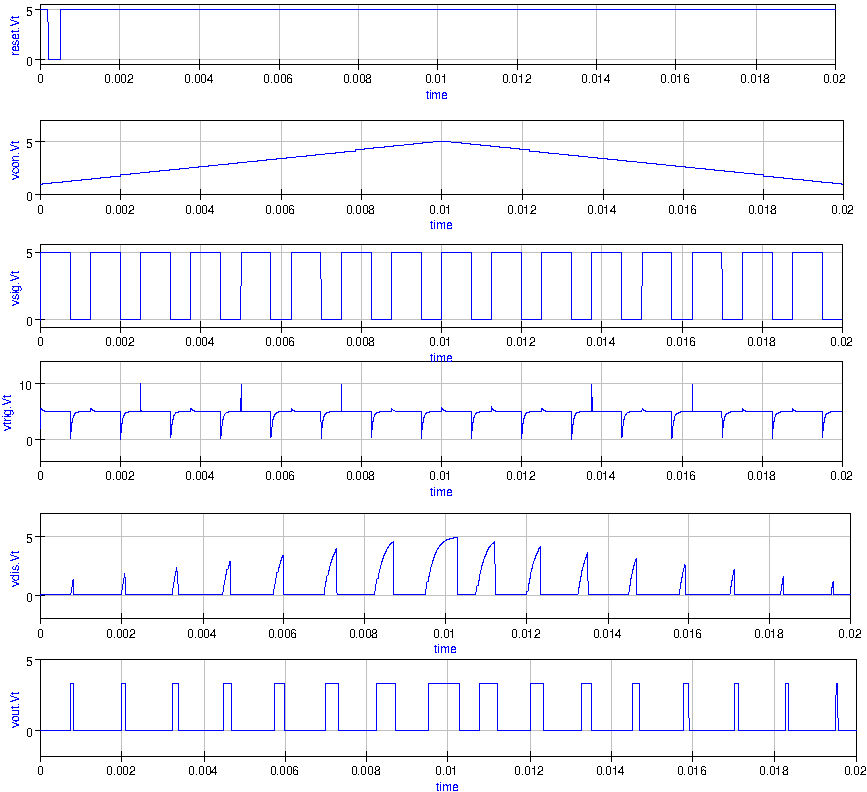
\includegraphics[width=1.0\linewidth]{555_timer_fig14}
  \caption{Simulation waveforms for pulse width modulator.}
  \label{fig:555_timer_fig14} 
\end{figure} 
\FloatBarrier

\tutsubsection{Pulse position modulation}
A pulse position modulator can be constructed from the astable waveform generator given in Fig.~\ref{fig:555_timer_fig9}. A modulating signal is applied to the control input pin 5 (CON); see Fig.~\ref{fig:555_timer_fig15}.  This signal causes the pulse position to vary with the amplitude of the applied modulating signal. A typical set of simulation waveforms for this circuit are shown in Fig.~\ref{fig:555_timer_fig16}. This is a very difficult circuit to simulate.  It is one case where the trapezoidal integration method works successfully whereas the 6th order Gear integration method appears to fail\footnote{The transient simulation never finishes and can only be terminated by clicking the simulation abort button.}.  Note that the trapezoidal results were obtained using 30000 points, Initial step = 0.001 nS, MinStep = 1e-16, MaxIter = 5000, abstol = 10uA and vntol = 10uV. 
\FloatBarrier
\begin{figure}[ht]
  \centering
  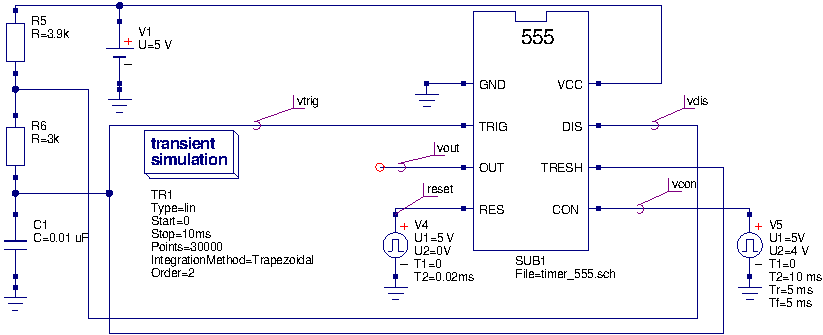
\includegraphics[width=1.0\linewidth]{555_timer_fig15}
  \caption{Pulse position modulator 555 timer circuit.}
  \label{fig:555_timer_fig15} 
\end{figure} 
\FloatBarrier

\FloatBarrier
\begin{figure}[ht]
  \centering
  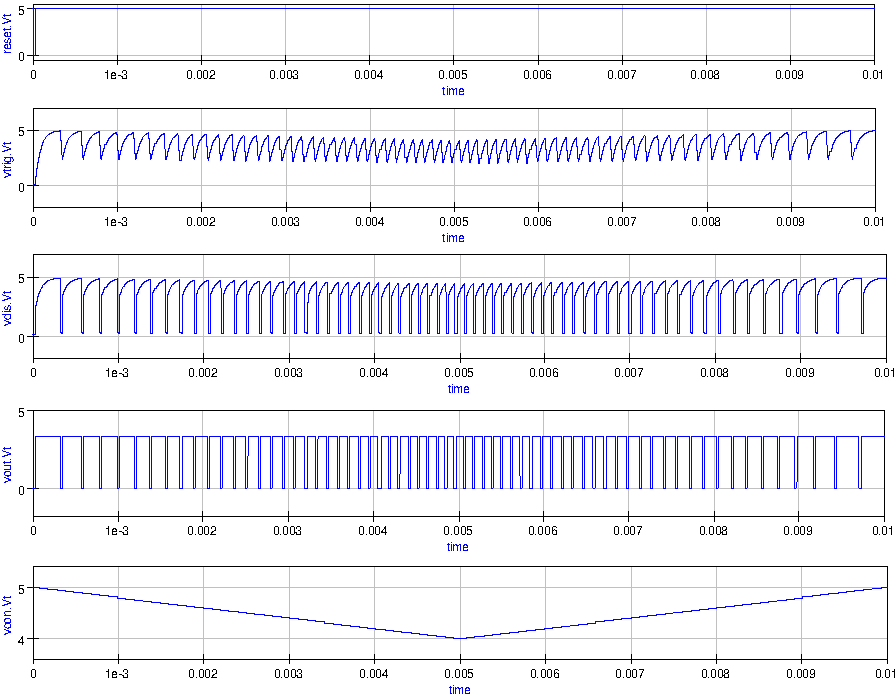
\includegraphics[width=1.0\linewidth]{555_timer_fig16}
  \caption{Simulation waveforms for pulse position modulator obtained using trapezoidal integration.}
  \label{fig:555_timer_fig16} 
\end{figure} 
\FloatBarrier


\addvspace{12pt}

\tutsection{Multiple 555 timer simulation examples}
Having established in the last section that the new Qucs 555 timer model can simulate the standard application circuits listed in a typical device data sheet, this part of the tutorial introduces two further, more complex, examples that demonstrate how the 555 timer is used in practice.

\tutsubsection{Sequential pulse train generation}
A very practical application of the 555 timer is the generation of timing pulses for control purposes. The circuit illustrated in Fig.~\ref{fig:555_timer_fig17} shows a set of monostable pulse generators connected in series and parallel. After circuit reset the falling edge of input pulse vin triggers the start of pulse sequence generation. The time duration of each monostable pulse is set by external capacitors C1 to C4\footnote{The pulse duration times set by C1 to C4, in Fig.~\ref{fig:555_timer_fig17}, have simply been chosen for demonstration purposes and do not represent any particular control timing sequence.}. The specification of the monostable pulse generator subcircuit is given in Fig.~\ref{fig:555_timer_fig18}. The sequential pulse generator is a complex circuit with:

    \begin{verbatim}
     60 R instances, 40 C instances, 4 VCVS instances, 1 Vdc instances,
     8 Idc instances, 2 Vpulse instances, 8 OpAmp instances, 4 Diode instances, 
     4 BJT instances, 8 Inv instances, 8 NOR instances and 4 OR instances. 
\end{verbatim} 

\FloatBarrier
\begin{figure}[ht]
  \centering
  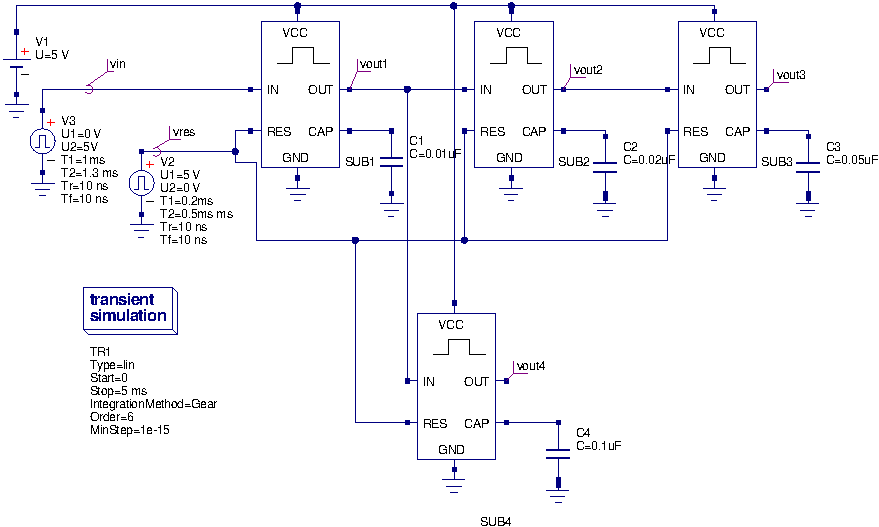
\includegraphics[width=1.0\linewidth]{555_timer_fig17}
  \caption{Sequential pulse generator circuit.}
  \label{fig:555_timer_fig17} 
\end{figure} 
\FloatBarrier

\FloatBarrier
\begin{figure}[ht]
  \centering
  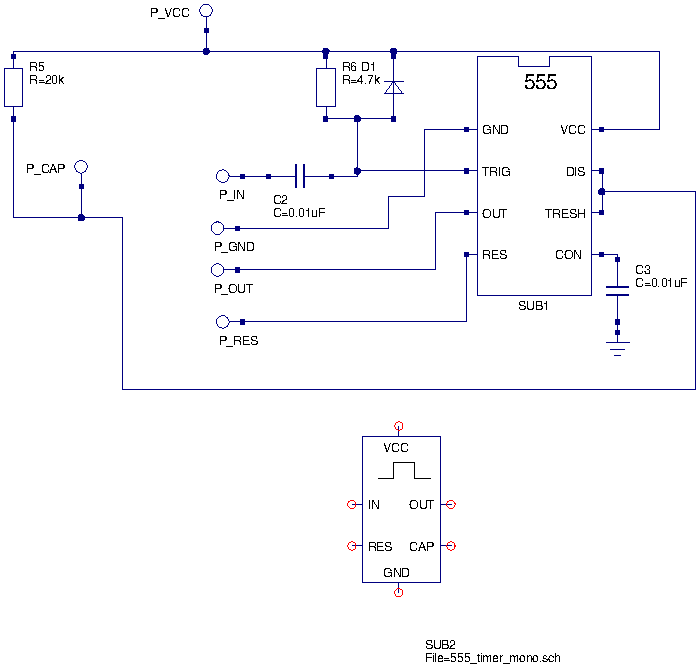
\includegraphics[width=1.0\linewidth]{555_timer_fig18}
  \caption{Monostable pulse generator subcircuit.}
  \label{fig:555_timer_fig18} 
\end{figure} 
\FloatBarrier

The large number of components, and indeed the complexity of the circuit, tend to make the simulation time of the pulse train generator circuit much greater than typical times recorded when simulating single 555 timer circuits.  Also, circuit DC convergence and transient analysis time step errors can be a problem, due to switching discontinuities, making careful selection of the non-linear diode parameters and the transient analysis conditions essential. In Fig.~\ref{fig:555_timer_fig18} a diode is used to clamp the 555 timer trigger input at five volts when the signal attempts to rise above 5 volts. The default Qucs diode parameters are similar to those specified by SPICE\footnote{The default values were set in an early version of SPICE, probably version 1, and appear to have not been changed as the simulator was developed.}.  By default the diode emission constant is set to 1 and the diode series resistance to zero ohms. Neither of these values are particularly representative for silicon diodes. For silicon devices, rather than germanium diodes, n needs to be between roughly 1.5 and 2.  Similarly, all diodes have some series resistance, often in the range 0.1 to 10 ohms depending on the power rating of the diode. To aid simulation these parameters have been set to n = 2 and Rs = 10$\Omega$. Figure.~\ref{fig:555_timer_fig19} illustrates a typical set of signal waveforms obtained from the simulation of the sequential pulse generator: the simulation conditions employed to generate these results are; Integration method = Gear, Order = 6, initialStep = 1 ns, MinStep = 1e-15, reltol = 0.001, abstol = 10$\mu$A, vntol = 10$\mu$V, Solver = CroutLU and initialDC = yes.

\FloatBarrier 
\begin{figure}[ht]
  \centering
  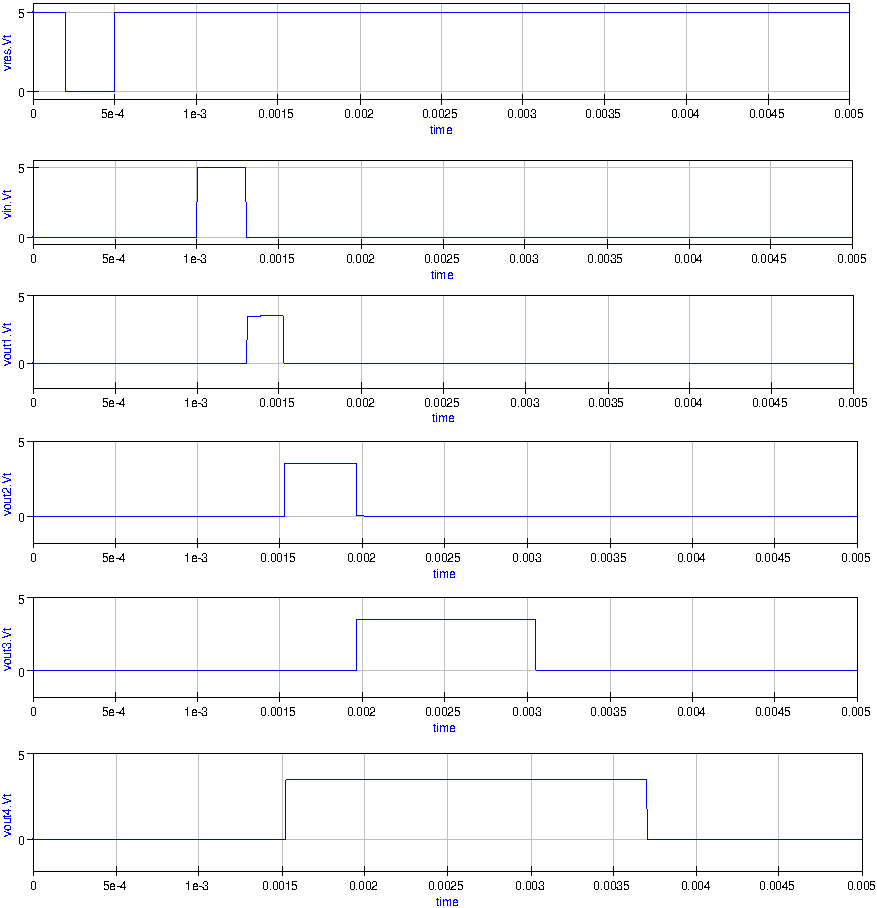
\includegraphics[width=1.0\linewidth]{555_timer_fig19}
  \caption{Simulation waveforms for the monostable pulse generator circuit.} 
  \label{fig:555_timer_fig19} 
\end{figure} 
\FloatBarrier

\tutsubsection{Frequency divider circuit}
A common requirement in both digital and mixed mode circuit design is frequency division, where a high frequency pulse train, often derived from a crystal controlled clock, is divided down to a much lower frequency\footnote{Often the resulting frequency is in the region 1 to 5 Hz and is used to flash an LED, or some other optical actuator, on/off.}. The classical way of dividing such signals is to use a chain of flip-flops each connected as a divide by two element.  The 555 timer can also be used for pulse train frequency division\footnote{555 timers are normally more efficient than flip-flops in this application because single devices can have divisors greater than two.}. The schematic shown in Fig.~\ref{fig:555_timer_fig20} shows a basic monostable mode 555 circuit with a train of pulses applied to the 555 trigger input pin 2 (TRIG). In an earlier section of these notes it was explained that the 555 trigger comparator input was signal level sensitive and retriggering takes place if the duration of the low signal section of the trigger waveform is greater than the monostable pulse duration.  In Fig.~\ref{fig:555_timer_fig20} the monostable pulse length is 0.22ms and rectangular voltage generator parameter TL is 0.5ms which causes retriggering to occur.  The effects of retriggering can be seen in Fig.~\ref{fig:555_timer_fig21}.  Frequency division employing 555 timers is based on the monostable circuit shown in Fig.~\ref{fig:555_timer_fig20} and hence circuit designers must make sure that retriggering does not take place. Illustrated in Fig.~\ref{fig:555_timer_fig22} is a two stage frequency division circuit where each stage divides the input pulse train by five giving an overall division ratio of twenty five.  The output waveforms for this circuit are shown in Fig.~\ref{fig:555_timer_fig23}. When designing 555 timer frequency divider circuits good performance can be achieved if the period of the 555 timer is set at (N-0.5) times the period of the input pulse train\footnote{E. A Parr, IC 555 Projects, Bernard Babani (publishing) Ltd, 1981, p. 109.}, where N is the division ratio and is in the range $2 \leq N \leq 10$.

\FloatBarrier
\begin{figure}[ht]
  \centering
  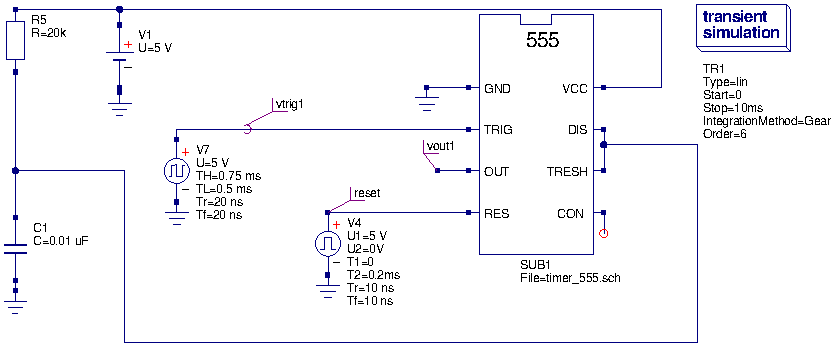
\includegraphics[width=1.0\linewidth]{555_timer_fig20}
  \caption{A monostable mode 555 timer circuit with a pulse train applied to the trigger input.}
  \label{fig:555_timer_fig20} 
\end{figure} 
\FloatBarrier 

\FloatBarrier
\begin{figure}[ht]
  \centering
  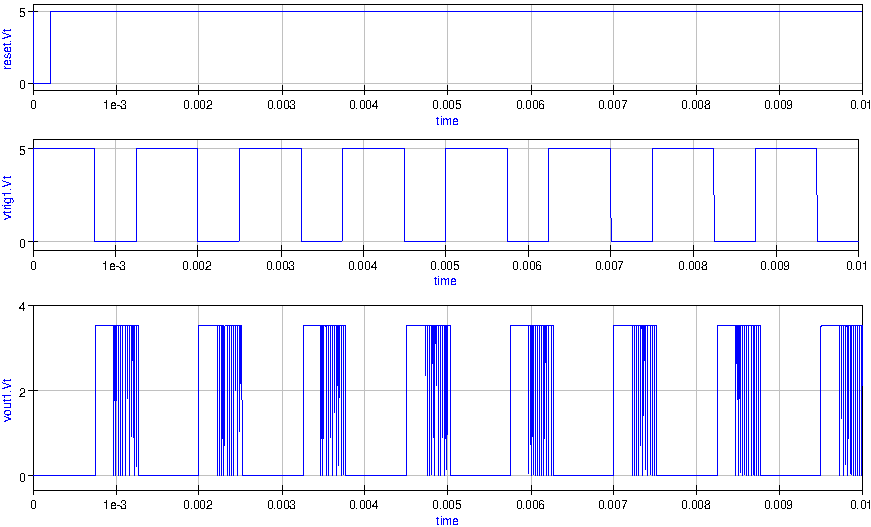
\includegraphics[width=1.0\linewidth]{555_timer_fig21}
  \caption{Simulation waveforms for the circuit given in Fig.~\ref{fig:555_timer_fig20}: these show 555 retriggering.}
  \label{fig:555_timer_fig21} 
\end{figure}  
\FloatBarrier 
\FloatBarrier 
\begin{figure}[ht]
  \centering
  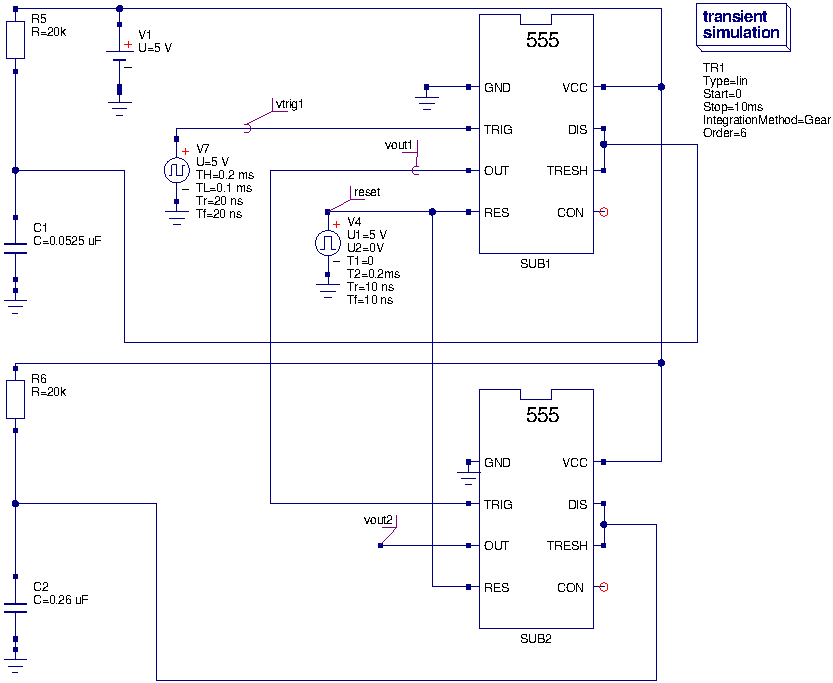
\includegraphics[width=1.0\linewidth]{555_timer_fig22} 
  \caption{A two stage 555 timer frequency division circuit.}
  \label{fig:555_timer_fig22}  
\end{figure} 
\FloatBarrier

\FloatBarrier
\begin{figure}[ht]
  \centering 
  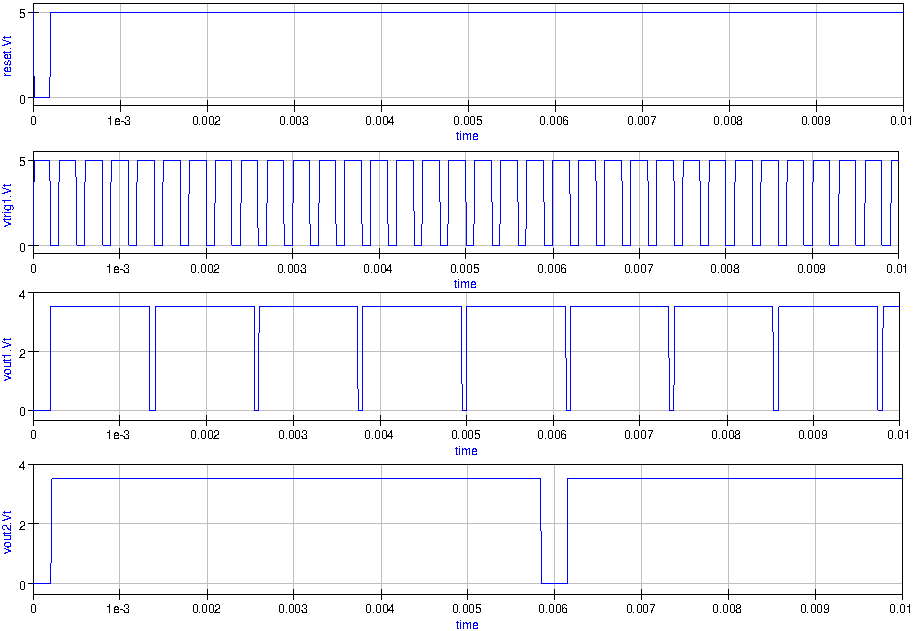
\includegraphics[width=1.0\linewidth]{555_timer_fig23} 
  \caption{Simulation waveforms for the circuit given in Fig.~\ref{fig:555_timer_fig22}.}
  \label{fig:555_timer_fig23}  
\end{figure} 
\FloatBarrier

\tutsection{End note}
Developing a simulation model for the 555 timer is an interesting challenge. This tutorial note attempts to describe the principles and macromodelling technology needed for such a task. It also demonstrates how much Qucs has matured as a universal simulator. The new Qucs 555 timer model is very much a first attempt on my part at building a functional model of this complex device.  Much more work needs to be done in the future to improve the 555 timer model. Low power 555 timer models are also needed for these popular variants.  Longer term a universal parameterised subcircuit model for the 555 timer should become possible once passing parameters to Qucs subcircuits and calculation of component values using equations are implemented. A special thanks to Stefan Jahn for all his encouragement and the many modifications he made to Qucs, which either corrected bugs or added functionality, during the period I have been working on this topic. 